\section{Convolutional Neural Networks}


In the field of machine learning, especially in the deep learning sector, a CNN is a deep learning algorithm. It can take an input image and reproduce an identification of the object with a certain probability. The special feature of a CNN is that it is able to learn filters of different types (e.g. horizontal lines, vertical lines, etc.). A convolutional neural network has a characteristic structure in terms of its layers. It is structured in convolutional, pooling, and fully connected layers. The arrangement of alternating convolutional and pooling layers allows a more accurate and complex analysis of the image. The first layers focus on shapes and colors, while later layers contribute to the identification of more complex details for the recognition of the overall image.

\subsection{Convolutional Layer}
The convolutional layer is the key component of a CNN. It contains a certain set of filters, also called kernels. The parameters of the filter are learned over the course of the training. The filter interacts with the image and convolves it. From this convolution, an activation map is created which is calculated from the dot product between each element of the filter and the input. The weights in the filter are maintained as the filter moves across the image. However, these weights adjust during backpropagation and the associated gradient descent to achieve the most accurate results. 

\begin{figure}[htb]
    \centering
    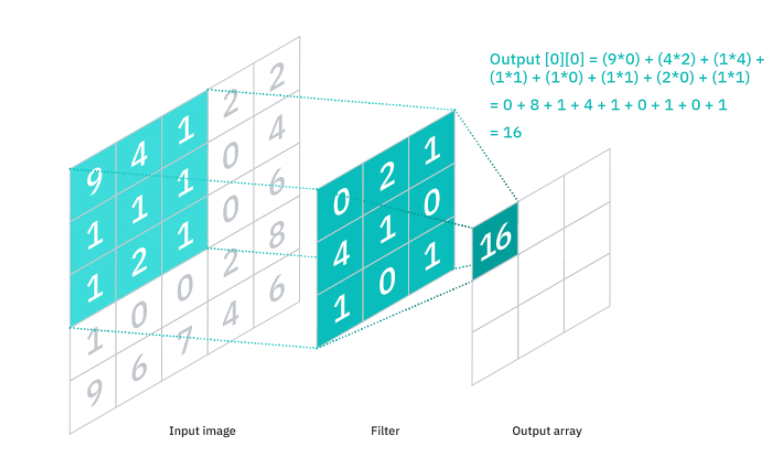
\includegraphics[width=7cm]{images/conv_layer.jpg}
    \caption{Convolutional Layer}
    \label{fig:convLayer}
\end{figure}

\subsection{Pooling Layer}
Since a great increase in dimension occurs through the use of a convolutional layer, a dimension reduction is required in the next step to reduce the number of parameters of a CNN. This is achieved by the pooling layer. It has the advantage that the computational cost decreases drastically. Also, unnecessary details are omitted, which is helpful for the later image identification.The most commonly used pooling methods are maximum and average pooling. In figure \ref{fig:poolingLayer}, you can see how a maximum pooling is performed, leading to a dimension reduction.

\begin{figure}[htb]
    \centering
    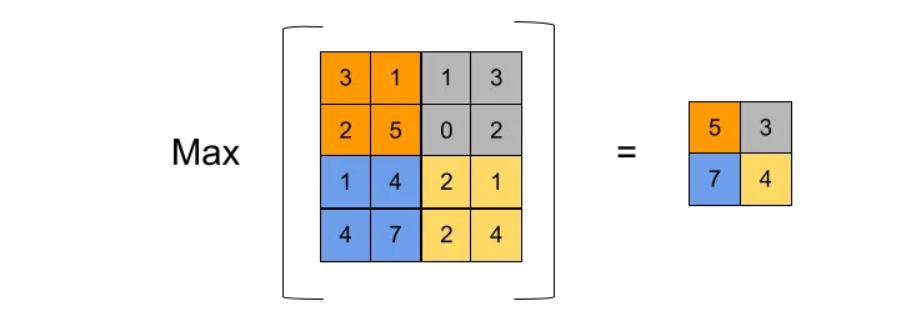
\includegraphics[width=7cm]{images/maxpooling.jpg}
    \caption{Max Pooling Layer}
    \label{fig:poolingLayer}
\end{figure}

\subsection{Fully-Connected Layer}
Since the individual pixel values of the input image are not directly connected to the output layer, a fully-connected layer is required which is directly connected to the output layer. The layer does the classification using the collected features from the previous layers. At the end, a softmax or Sigmoid function (dependent on the problem) is applied, which outputs a classification using probabilities between 0 and 1.

\begin{figure}[htb]
    \centering
    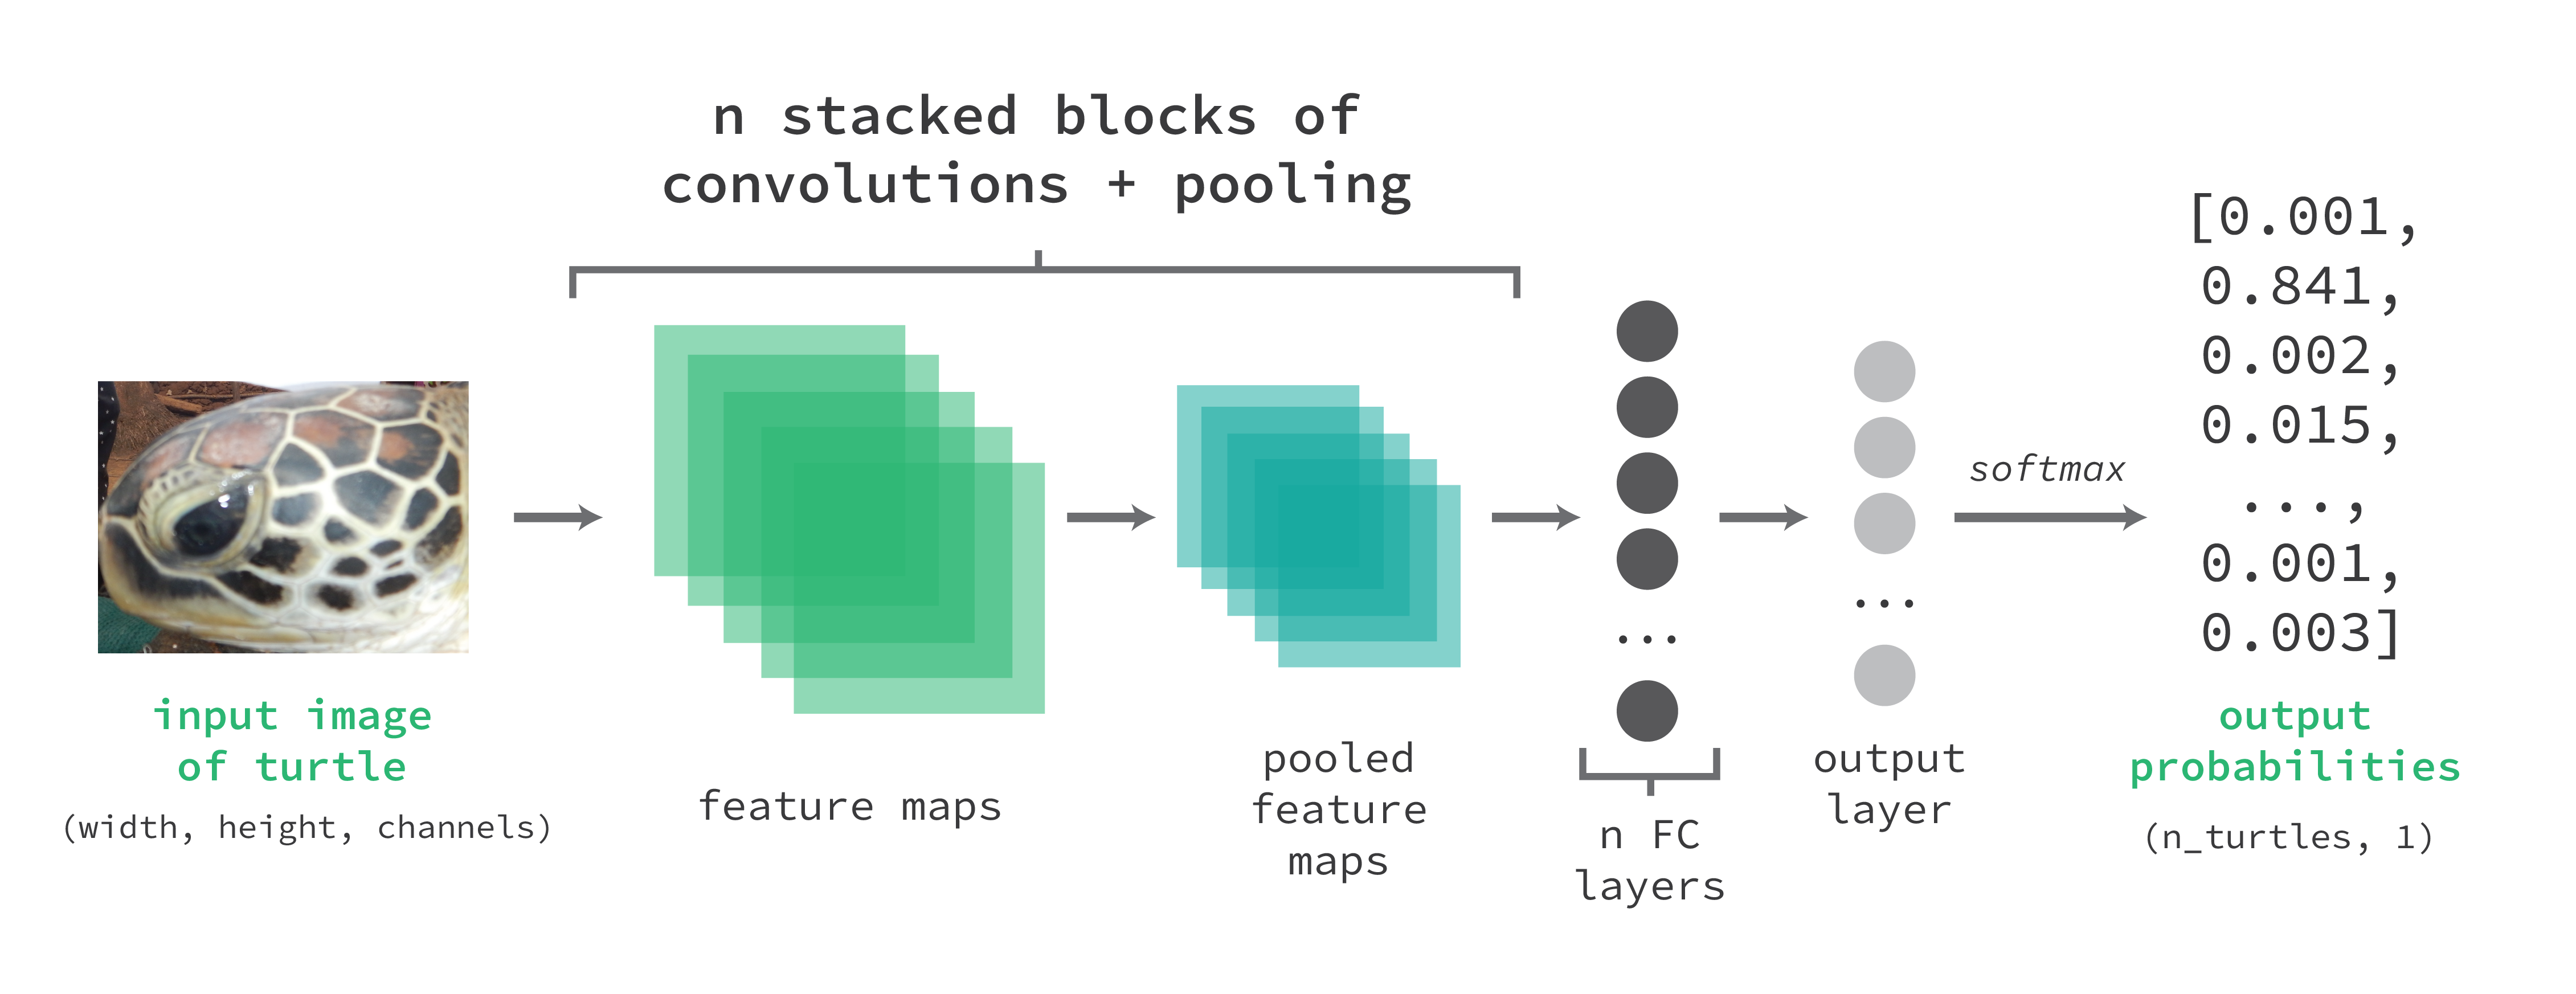
\includegraphics[width=10cm]{images/cnn_turtle_pooling.png}
    \caption{Turtle Image using CNN}
    \label{fig:turtleCNN}
\end{figure}